%% Springer Nature LaTeX template (sn-jnl, v3.1), numbered references (sn-mathphys-num).
%% Build: tectonic -X compile main.tex   (or pdflatex + bibtex on Overleaf).
\documentclass[pdflatex,sn-mathphys-num,iicol]{sn-jnl}

\usepackage{graphicx}
\usepackage{multirow}
\usepackage{amsmath,amssymb,amsfonts}
\usepackage{amsthm}
\usepackage[title]{appendix}
\usepackage{xcolor}
\usepackage{textcomp}
\usepackage{booktabs}
\usepackage{algorithm}
\usepackage{algpseudocode}
\usepackage{tikz}
\usetikzlibrary{arrows.meta,positioning,fit,calc}
\usepackage{siunitx}
\usepackage{url}

\newcommand{\RI}{\mathrm{RI}^{*}}
\raggedbottom

\begin{document}

\title[Forecasting time to choke restriction from mineral scale]{Forecasting Time to Choke Restriction from Mineral Scale with Production Sensors: A Physics-Informed Survival Model and an Unseen-Well Benchmark on the 3W Dataset}

\author*[1]{\fnm{Muhammad} \sur{Haseeb}}\email{EMAIL-HASEEB@nu.edu.pk}
\author[1]{\fnm{Muavia} \sur{Shakeel}}\email{EMAIL-MUAVIA@nu.edu.pk}
\affil*[1]{\orgname{National University of Computer and Emerging Sciences (FAST-NUCES)}, \orgaddress{\city{Islamabad}, \country{Pakistan}}}

\abstract{Mineral scale that narrows the production choke of an oil well grows over hours to weeks, yet it is
usually noticed late from trend charts. Machine-learning studies on the public Petrobras 3W dataset detect
such events once they have begun, mostly with the same wells in training and test sets, and none forecasts
when the restriction becomes critical. This paper formulates choke-scale forecasting as discrete-time
survival analysis: from each 6-h window of 1-min production-sensor data, a model estimates the probability
that a self-referenced restriction index rises by 5\,\% within horizons of 1 to 72~h, with censored
instances handled explicitly. The proposed model, PI-PatchSurv, fuses a channel-independent patch
Transformer with a physics-feature branch through a learned gate and outputs a monotone risk curve; it is
trained with a censoring-aware likelihood and a monotonicity penalty, and its uncertainty is quantified with
a five-member ensemble and split-conformal intervals. Twelve models were compared on 3W version 2.0.0 by
leave-one-well-out validation (24 real events in six wells), with alarm thresholds fixed on separate
calibration wells. Recurrent forecasters ranked events best, with an area under the precision--recall
curve at 24~h of up to 0.74 against 0.53 for a physics threshold rule, and caught up to 17 of 24 events a
median of 2.9~h ahead. PI-PatchSurv ranked lower (0.64) but gave the best-calibrated intervals (coverage
0.87 at the 90\,\% level against 0.33--0.54), the smallest time-to-event error (6.8~h) and no loss when
three of nine sensors failed. Forecasting the time to choke restriction on unseen wells is therefore
feasible, with lead times bounded by the short recordings.
}

\keywords{mineral scale, production choke, time-to-event forecasting, discrete-time survival analysis, physics-informed deep learning, 3W dataset}

\maketitle

\section{Introduction}\label{sec:intro}

Inorganic scale such as calcium carbonate and barium sulphate precipitates when produced water becomes
supersaturated, for example when pressure falls and CO$_2$ leaves solution or when injected and formation
waters mix \citep{kamal2018,olajire2015}. Inside a production choke the deposit narrows the throat, raises
the upstream pressure and forces the operator to choke the well back; left untreated it ends in an
unplanned cleaning or acid job and deferred production. Because scale grows gradually, over hours to
weeks, a forecast of \emph{when} the restriction will become critical would allow the intervention to be
planned rather than improvised. In practice the restriction is still tracked manually from trend charts,
which makes choke scaling a natural target for the data-driven predictive maintenance that is now common in
manufacturing and process industries.

Public data for this problem became available with the 3W dataset released by Petrobras
\citep{vargas2019,vargas2026}, which contains labelled multivariate sensor series of real, simulated and
hand-drawn undesirable events in offshore wells, among them scaling in the production choke. The
machine-learning work on 3W has, however, treated the task almost exclusively as detection: a model
classifies whether an event is under way, usually after it has started \citep{aranha2024,lopes2025,lopes2026}.
Detection answers whether the well is scaling now, not how long it will take until the restriction becomes
critical. Evaluations also commonly split windows or instances at random, so that windows of the same well
appear in training and test sets; a recent community proposal for 3W shows that the macro-F1 score falls
from 0.99 under a random split to 0.30 when whole wells are held out \citep{issue231}. Outside 3W, the
data-driven studies that estimate the magnitude of scale rely on simulated well histories or on water
chemistry rather than on production-sensor streams of real wells
\citep{cheng2022,askar2025,su2024,molina2025}, and few studies attach calibrated uncertainty to their
outputs, although an alarm that is right on average but uncalibrated on a new well is of little use to an
operator. To the best of our knowledge, no published study forecasts the time to a critical level of choke
scaling from production sensors, evaluates such a forecast on wells never seen in training, or reports its
uncertainty.

This paper addresses that gap. Choke-scale forecasting is cast as discrete-time survival analysis, in which
every window of sensor data receives the probability that the restriction reaches a critical level within
horizons of 1 to 72~h and instances that never reach it are treated as right-censored. Because the
pressure downstream of the choke is missing in all real scaling instances of 3W, the restriction is measured
by an index normalised to each instance's own early baseline, which serves both as label and as causal input
and makes wells of very different pressure comparable. On this formulation we build PI-PatchSurv, a
channel-independent patch Transformer whose sequence representation is fused through a learned gate with a
branch of physics features and decoded by a survival head that yields a monotone risk curve; a monotonicity
loss, a deep ensemble and split-conformal intervals complete the model. The approach is evaluated against
eleven alternatives, from a physics threshold rule to re-implementations of the architectures of the base
studies, on leave-one-well-out folds in which every threshold and hyper-parameter is chosen on separate
calibration wells.

The novelty of this research lies in three aspects. First, it provides, as far as we are aware, the first
time-to-event formulation of an undesirable event in the 3W dataset, together with a self-referenced
restriction proxy that makes the formulation usable when the downstream sensors are missing. Second, it
combines learned sequence features, physical indicators and calibrated uncertainty in one survival model
for well operations. Third, it reports an unseen-well benchmark of twelve models with fixed and tuned
hyper-parameters, event-level alarm metrics, robustness tests and a dataset-version generalisation test, and
documents two pitfalls of 3W version 2.0.0 that silently change results. The results show that
time-to-restriction forecasting on unseen wells is feasible but that its lead time is bounded by the data,
and that simple recurrent forecasters rank events as well as the proposed model, whose advantages lie in
uncertainty quality and robustness.

The remainder of this paper is organised as follows. Section~\ref{sec:related} reviews related work, and
Section~\ref{sec:method} presents the proposed method. Section~\ref{sec:setup} describes the experimental
setup, Section~\ref{sec:results} reports the results, Section~\ref{sec:comparison} compares them with the
base studies, and Section~\ref{sec:ablation} presents the ablation study. Section~\ref{sec:discussion}
discusses implications and limitations, and Section~\ref{sec:conclusion} concludes the paper.

\section{Related work}\label{sec:related}

\subsection{Event detection on the 3W dataset}

The 3W dataset was introduced with benchmarks for detecting eight types of undesirable events
\citep{vargas2019}, and version 2.0.0 extends it to nine event types and 2,228 instances \citep{vargas2026}.
Detection approaches range from autoencoders combined with rule-based decision diagrams, which report
true-positive rates above 90\,\% in the early stages of an anomaly \citep{aranha2024}, to Transformer
detectors for intelligent completions \citep{aranha2025} and open-world pipelines that combine
reconstruction, binary classifiers and clustering \citep{lopes2025}. A recent layer of large-language-model
agents on top of such a pipeline reports a novelty-detection rate of 94.9\,\% for choke scaling on 3W
segments \citep{lopes2026}. These studies recognise an event that has begun, but none outputs a lead time,
and most do not separate wells between training and test sets; a held-out-well benchmark for 3W has only
recently been proposed \citep{issue231}.

\subsection{Data-driven prediction of mineral scale}

Outside 3W, deep networks detect scale build-up and estimate its magnitude from simulated well histories with
more than 95\,\% detection accuracy \citep{cheng2022}, artificial neural networks predict sulphide-scale
deposition from water analyses and operating data \citep{askar2025}, back-propagation networks estimate the
risk of wellbore blockage from water chemistry in tight gas fields \citep{su2024}, and machine-learning
surrogates reproduce the saturation indices of PHREEQC \citep{parkhurst2013} from a few water properties
\citep{molina2025}. These works establish that scale is predictable from chemistry or from simulated
histories, but they do not use real production-sensor streams, do not forecast the time to a critical
state and are not evaluated on unseen wells.

\subsection{Sequence models and time-to-event learning}

Recurrent networks such as the long short-term memory (LSTM) network \citep{hochreiter1997} and the gated
recurrent unit (GRU) \citep{cho2014}, temporal convolutional networks \citep{bai2018}, attention models
\citep{vaswani2017}, patch-based Transformers \citep{nie2023} and inverted Transformers \citep{liu2024itrans}
are standard tools for multivariate sensor series. A hybrid Transformer--LSTM forecasts water breakthrough in
gas wells two to six days ahead and transfers between similar wells \citep{lai2026}, which makes it the
closest forecasting study of a well event with a lead time. Discrete-time survival heads
\citep{gensheimer2019,kvamme2021} and their deep variants \citep{lee2018deephit} handle censoring and give
monotone risk curves, but they have not been applied to the forecasting of well events. Physics-informed
learning injects domain knowledge through features, architecture or loss terms
\citep{karniadakis2021,willard2022}, while deep ensembles \citep{lakshminarayanan2017} and conformal
prediction \citep{angelopoulos2023} provide uncertainty estimates.

Table~\ref{tab:related} summarises the closest studies. The present work differs from them in four
respects: it forecasts the time to a critical level rather than detecting an event, it uses real
production-sensor data of the choke, it evaluates on wells excluded from training with thresholds fixed in
advance, and it reports calibrated, interval-valued uncertainty.

\begin{table}[t]
\caption{Summary of the closest related studies}
\label{tab:related}
\footnotesize\setlength{\tabcolsep}{3pt}
\begin{tabular*}{\textwidth}{@{\extracolsep\fill}p{2.5cm}p{2.6cm}p{1.9cm}cccp{1.5cm}}
\toprule
Study & Task & Data & Sens. & TTE & HO & Unc. \\
\midrule
\citet{vargas2019,vargas2026} & Event-detection benchmark & 3W & yes & no & no & no \\
\citet{aranha2024} & Anomaly detection & Field wells & yes & no & n/s & no \\
\citet{lopes2025} & Open-world detection & Well completions & yes & no & n/s & no \\
\citet{lopes2026} & Detection, explanation & 3W & yes & no & no & Wilson CI \\
3W proposal \citep{issue231} & Classification benchmark & 3W & yes & no & yes & Bootstrap \\
\citet{cheng2022} & Scale magnitude & Simulated wells & yes & no & no & no \\
\citet{askar2025} & Sulphide-scale risk & Field chemistry & no & no & n/s & no \\
\citet{molina2025} & Saturation-index surrogate & Produced water & no & no & n/s & no \\
\citet{lai2026} & Breakthrough forecast & 9 gas wells & yes & days & partly & no \\
This work & Time to $+5\,\%$ restriction & 3W & yes & yes & yes & Ensemble, conformal \\
\botrule
\end{tabular*}
\footnotetext{Sens.: production-sensor data; TTE: time-to-event forecast; HO: whole wells held out of training; n/s: not stated in the
accessible abstract; Unc.: uncertainty quantification.}
\end{table}

\section{Proposed methodology}\label{sec:method}

\subsection{Problem formulation}\label{sec:formulation}

Let $\mathbf{x}_{1:T}\in\mathbb{R}^{T\times C}$ be the 1-minute sensor series of one instance with $C$
channels and $\mathbf{m}_{1:T}\in\{0,1\}^{T\times C}$ the corresponding mask, where $m_{t,c}=1$ marks a
missing or frozen value. Let $p_t$ denote the pressure upstream of the production choke (P-MON-CKP) and
$t_0$ the onset of scaling, i.e.\ the first minute labelled as transient or steady class~7. Because the
downstream pressure and the choke opening are missing in the real class-7 instances
(Section~\ref{sec:data}), the pressure drop across the choke cannot be computed. We therefore define the
self-referenced restriction index
\begin{align}
\RI_t&=\frac{p_t}{\operatorname{median}\{p_s : s<t_0\}},\label{eq:ri}\\
\widetilde{\RI}_t&=\frac{p_t}{\operatorname{median}\{p_s : s\le 60\}},\nonumber
\end{align}
where $\RI_t$ (pre-onset baseline) defines the label and $\widetilde{\RI}_t$ (median of the first hour,
always before onset and therefore causal) is used as an input feature. The event time $t_E$ is the first
minute after $t_0$ at which the 60-minute rolling median of $\RI_t$ reaches $1.05$, i.e.\ the restriction
has grown by $5\,\%$.

A forecast is issued for windows $\mathbf{w}_t=(\mathbf{x},\mathbf{m})_{t-L+1:t}$ of length $L=360$~min,
every 10~min. For $t<t_E$ the time-to-event is $\tau_t=t_E-t$, discretised into $K=7$ bins by the
horizons $\mathcal{H}=\{1,3,6,12,24,72\}$~h (the last bin is $>72$~h). Windows of normal instances, of
other event classes and of class-7 instances that never cross $1.05$ are right-censored at the end of the
instance; windows after $t_E$ are discarded. The model outputs a cumulative risk
$F_t(k)=P(\tau_t\le h_k\mid \mathbf{w}_t)$ for each horizon $h_k\in\mathcal{H}$.

\subsection{Architecture}

Figure~\ref{fig:arch} shows PI-PatchSurv. It has a sequence branch, a physics branch, a gated fusion and a
discrete-time survival head.

\begin{figure*}[t]
\centering
\resizebox{\textwidth}{!}{%
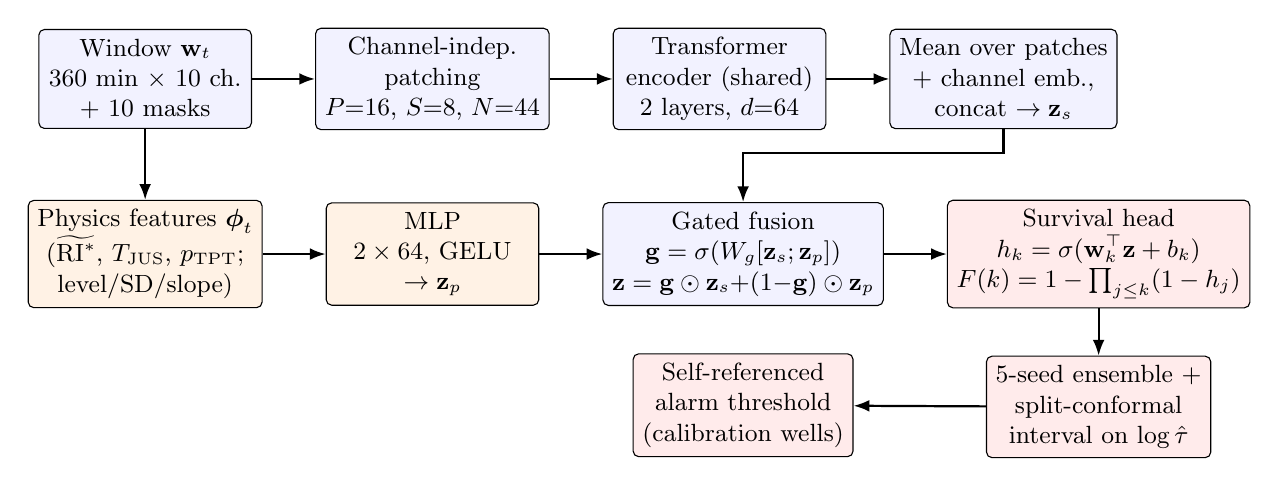
\begin{tikzpicture}[
  font=\small, node distance=6mm and 8mm,
  box/.style={draw, rounded corners=2pt, align=center, minimum height=11mm, minimum width=27mm, fill=blue!5},
  phy/.style={box, fill=orange!10}, outb/.style={box, fill=red!8},
  arr/.style={-{Latex[length=2mm]}, thick}]
% row 1: sequence branch
\node[box] (in) {Window $\mathbf{w}_t$\\ 360 min $\times$ 10 ch.\\ + 10 masks};
\node[box, right=of in] (patch) {Channel-indep.\\ patching\\ $P{=}16$, $S{=}8$, $N{=}44$};
\node[box, right=of patch] (enc) {Transformer\\ encoder (shared)\\ 2 layers, $d{=}64$};
\node[box, right=of enc] (pool) {Mean over patches\\ + channel emb.,\\ concat $\rightarrow \mathbf{z}_s$};
% row 2: physics branch, fusion, head
\node[phy, below=9mm of in] (feat) {Physics features $\boldsymbol{\phi}_t$\\ ($\widetilde{\RI}$, $T_{\mathrm{JUS}}$, $p_{\mathrm{TPT}}$;\\ level/SD/slope)};
\node[phy, right=of feat] (mlp) {MLP\\ $2\times 64$, GELU\\ $\rightarrow \mathbf{z}_p$};
\node[box, right=of mlp] (gate) {Gated fusion\\ $\mathbf{g}=\sigma(W_g[\mathbf{z}_s;\mathbf{z}_p])$\\ $\mathbf{z}=\mathbf{g}\odot\mathbf{z}_s{+}(1{-}\mathbf{g})\odot\mathbf{z}_p$};
\node[outb, right=of gate] (head) {Survival head\\ $h_k=\sigma(\mathbf{w}_k^{\top}\mathbf{z}+b_k)$\\ $F(k)=1-\prod_{j\le k}(1-h_j)$};
\node[outb, below=6mm of head] (unc) {5-seed ensemble +\\ split-conformal\\ interval on $\log\hat\tau$};
\node[outb, below=6mm of gate] (alarm) {Self-referenced\\ alarm threshold\\ (calibration wells)};
\draw[arr] (in) -- (patch); \draw[arr] (patch) -- (enc); \draw[arr] (enc) -- (pool);
\draw[arr] (in) -- (feat); \draw[arr] (feat) -- (mlp); \draw[arr] (mlp) -- (gate);
\draw[arr] (pool.south) -- ++(0,-3mm) -| (gate.north);
\draw[arr] (gate) -- (head); \draw[arr] (head) -- (unc); \draw[arr] (unc) -- (alarm);
\end{tikzpicture}}
\caption{PI-PatchSurv. Each sensor channel is cut into overlapping patches; a channel-independent Transformer
encodes the patches (each mask is folded into its value token). Engineered physics features pass through an
MLP. A learned gate fuses both representations, and a discrete-time survival head outputs a risk curve that
is monotone in the horizon. Uncertainty comes from a deep ensemble and split-conformal intervals.}
\label{fig:arch}
\end{figure*}

\textbf{Sequence branch.} Following PatchTST~\cite{nie2023}, every channel $c$ of the window is split into
$N=\lfloor (L-P)/S\rfloor+1=44$ overlapping patches of length $P=16$ with stride $S=8$. The value patch and
its mask patch are concatenated into a $2P$-dimensional token, linearly embedded to $d=64$ and given a
learned positional embedding. A two-layer Transformer encoder~\cite{vaswani2017} with four heads, shared
across channels, encodes the tokens; the patch outputs of each channel are averaged, a learned channel
embedding is added, and the channel vectors are concatenated and projected to $\mathbf{z}_s\in\mathbb{R}^d$.
Channel independence shares parameters across sensors, which matters with few events, and folding masks
into tokens lets the model discount imputed segments.

\textbf{Physics branch.} The feature vector $\boldsymbol{\phi}_t\in\mathbb{R}^{36}$ contains the rolling
mean, standard deviation and least-squares slope over 10, 60 and 360~min of $\widetilde{\RI}$, of the
upstream choke pressure, of the upstream choke temperature $T_{\mathrm{JUS}}$ (Joule--Thomson cooling grows as
the throat narrows) and of the production-tubing pressure $p_{\mathrm{TPT}}$ (a system-wide rise moves it
too, a choke restriction does not). A two-layer MLP with GELU and dropout 0.1 maps $\boldsymbol{\phi}_t$ to
$\mathbf{z}_p\in\mathbb{R}^d$. In the \emph{-SI} variant, two saturation indices (calcite, barite) computed by
PHREEQC~\cite{parkhurst2013} at the window's temperature and pressure for public Gulf-of-Mexico brines
\cite{blondes2023} are appended to $\boldsymbol{\phi}_t$.

\textbf{Gated fusion and survival head.} The gate
$\mathbf{g}=\sigma(W_g[\mathbf{z}_s;\mathbf{z}_p]+\mathbf{b}_g)$ forms
$\mathbf{z}=\mathbf{g}\odot\mathbf{z}_s+(1-\mathbf{g})\odot\mathbf{z}_p$, where $\sigma$ is the logistic
function and $\odot$ the element-wise product. The head~\cite{gensheimer2019,kvamme2021} gives a hazard per
bin, $h_k=\sigma(\mathbf{w}_k^{\top}\mathbf{z}+b_k)$, and the cumulative risk
\begin{equation}
F(k)=1-\prod_{j=1}^{k}(1-h_j),\qquad k=1,\dots,K,
\label{eq:cdf}
\end{equation}
which is non-decreasing in $k$ by construction.

\subsection{Training objective}

For window $i$ with bin index $k_i$ (the event bin if an event is observed, $\delta_i=1$, otherwise the bin
in which observation ends, $\delta_i=0$), the censor-aware log-likelihood is
\begin{align}
\ell_i&=\sum_{j<k_i}\log(1-h_{ij})+\delta_i\log h_{ik_i},\nonumber\\
\mathcal{L}_{\mathrm{surv}}&=-\frac{\sum_i \omega_i\,\ell_i}{\sum_i \omega_i},
\label{eq:nll}
\end{align}
so a censored window is only credited with surviving the bins before $k_i$. The weight $\omega_i$ equals the
ratio of censored to event windows (clipped to $[1,100]$) for event windows and 1 otherwise, which
compensates the rarity of events. Scale does not shrink without an intervention, so on consecutive windows
$(t-10,t)$ of the same class-7 instance a monotonicity term penalises drops of the forecast risk:
\begin{align}
\mathcal{L}_{\mathrm{mono}}&=\frac{1}{|\mathcal{P}|K}\sum_{(t-10,t)\in\mathcal{P}}\sum_{k=1}^{K}\nonumber\\
&\qquad\max\{0,\,F_{t-10}(k)-F_t(k)\},\nonumber\\
\mathcal{L}&=\mathcal{L}_{\mathrm{surv}}+\lambda\,\mathcal{L}_{\mathrm{mono}},
\label{eq:loss}
\end{align}
with $\lambda=0.1$. Algorithm~\ref{alg:train} summarises training and inference.

\begin{algorithm*}[t]
\caption{Training and deployment of PI-PatchSurv for one leave-one-well-out fold}\label{alg:train}
\footnotesize
\begin{algorithmic}[1]
\Require training wells $\mathcal{D}_{\mathrm{tr}}$ (real + synthetic), calibration wells $\mathcal{D}_{\mathrm{ca}}$ (real), test wells $\mathcal{D}_{\mathrm{te}}$ (real)
\State fit robust scaling (median, IQR) on $\mathcal{D}_{\mathrm{tr}}$ only
\For{seed $r=1,\dots,R$}
  \For{epoch $=1,\dots,12$}
    \For{step $=1,\dots,150$}
      \State sample a batch of 256 windows from $\mathcal{D}_{\mathrm{tr}}$; compute $\mathcal{L}$ (Eq.~\ref{eq:loss}); AdamW update
    \EndFor
    \State keep the weights with the lowest $\mathcal{L}_{\mathrm{surv}}$ on $\mathcal{D}_{\mathrm{ca}}$ \Comment{early stopping}
  \EndFor
\EndFor
\State ensemble: $\bar F(k)=\frac{1}{R}\sum_r F^{(r)}(k)$
\State threshold $\theta$ on $\mathcal{D}_{\mathrm{ca}}$: largest recall with $\le 1$ false alarm per well-month,
\Statex \hspace{\algorithmicindent} on the score $\bar F_t(h_{24})-\operatorname{median}_{s\le 60}\bar F_s(h_{24})$
\State conformal quantile $q$ of $|\log\tau-\log\hat\tau|$ on event windows of $\mathcal{D}_{\mathrm{ca}}$ at level 90\,\%
\State on $\mathcal{D}_{\mathrm{te}}$: alarm when the self-referenced score exceeds $\theta$; interval $[\hat\tau e^{-q},\hat\tau e^{q}]$
\end{algorithmic}
\end{algorithm*}

\subsection{Uncertainty and deployment}

Five seeds are averaged as a deep ensemble~\cite{lakshminarayanan2017}. The predicted median time-to-event
$\hat\tau$ is the horizon at which $\bar F$ reaches $0.5$ (log-interpolated), and a split-conformal
interval~\cite{angelopoulos2023} is calibrated on the event windows of the calibration wells. Alarm
thresholds are set on the calibration wells for at most one false alarm per well-month. Because absolute
score levels differ between wells, the deployed alarm uses the score minus its median over the instance's
first hour (\emph{calib-self}), the score-space analogue of $\widetilde{\RI}$; the raw score
(\emph{calib}) is reported for comparison.

\subsection{Changes after the Phase~2 review}

The design was reviewed before implementation; the review raised no objections, and the following changes
were forced by the data or by compute. (i) The target changed from the onset of scaling to its severity
($+5\,\%$), because real instances contain a median of only 6.5~h of normal operation before onset.
(ii) The planned restriction index based on the pressure drop across the choke was replaced by $\RI$
(Eq.~\ref{eq:ri}), since the downstream pressure is missing in all real class-7 instances. (iii) The
generalisation test was corrected from 21 to 18 wells in 3W v1.1.1. (iv) The produced-water database
version 2.3 could not be downloaded, and version 3.0~\cite{blondes2023} was used. (v) The ``no patching''
ablation uses gradient accumulation to fit in memory (Section~\ref{sec:ablation}).

\section{Experimental setup}\label{sec:setup}

\subsection{Dataset}\label{sec:data}

We use 3W v2.0.0 \citep{vargas2026} pinned to repository commit \texttt{826fec4} \citep{petrobras3w}: 2,228
instances sampled at 1~Hz, of which 1,119 are real (40 wells), 1,089 simulated and 20 hand-drawn. Class~7
(\emph{scaling in the production choke}) has 36 real instances from six wells (well~24: 19, 22: 8,
23: 4, 21: 2, 6: 2, 1: 1) and 10 hand-drawn ones; there are no simulated class-7 instances. In 31 of the
36 real instances the label never leaves the transient state, so onset is defined by the first transient
or steady label. The pressure downstream of the choke and the downstream temperature are missing in all
real class-7 instances and the choke opening in 78\,\%, which rules out a pressure-drop restriction
index. Under the $+5\,\%$ criterion, 24 of the 36 real instances reach the event (well~24: 17, 22: 3,
6: 2, 1: 1, 21: 1, 23: 0); the median time from a window to the event is 12~h (maximum 147~h).

\subsection{Preprocessing and features}

Signals are averaged to one-minute resolution. Values constant for more than 30~min while the well is
open (frozen sensors) and missing values become mask channels; gaps of up to 10~min are forward-filled;
values with $|x|>10^9$ (sentinel readings) are treated as missing. Variables missing in more than half of
the real instances are dropped, leaving nine channels (upstream choke pressure and temperature, tubing
pressure and temperature, annulus pressure, downhole pressure and temperature, gas-lift line pressure and
the safety-valve state) plus $\widetilde{\RI}$. Robust scaling (median, inter-quartile range) is fitted on
the training files of each fold only. Two data issues of 3W were corrected: (i) 225 file names, covering
885 synthetic instances, repeat across class folders, so instances are keyed by class and file name; and
(ii) hand-drawn pressures are about $10^5$ times smaller than real ones (bar instead of Pa) and are
converted. Windows are formed every 10~min after the first hour, giving 109,547 windows (44,386 real).

\subsection{Splits}

We use six leave-one-well-out folds, one per well with real scaling. In each fold the \emph{test} set
contains all real instances of the held-out scaling well plus a rotating group of wells without scaling,
so every real instance is tested exactly once (24 events, about 248 negative well-days in total). The
\emph{calibration} set contains the next scaling well that has an event (never well~24, which holds 17 of
the 24 events) plus another group of non-scaling wells; it is used for early stopping, hyper-parameter
tuning, alarm thresholds and conformal calibration. The \emph{training} set contains the remaining real
wells and all simulated and hand-drawn instances; synthetic data never enters calibration or test. For the
generalisation test we train on the wells present in 3W v1.1.1 (18 real wells; 4 training events)
and test on wells added in v2.0.0 (wells 22--24, 20 events).

\subsection{Baselines}

All baselines receive the same windows. B0 is a physics rule that thresholds the 60-minute mean of
$\widetilde{\RI}$. B1 (logistic regression) and B2 (gradient-boosted trees \citep{friedman2001}, scikit-learn
\citep{pedregosa2011}) use 63 tabular features at the window end. The deep baselines use per-horizon
binary cross-entropy heads and the same training budget and early stopping as PI-PatchSurv: B3 LSTM
\citep{hochreiter1997}, B4 GRU \citep{cho2014}, B5 CNN-LSTM, B6 TCN \citep{bai2018}, B7 the hybrid
Transformer--LSTM of \citet{lai2026}, B8 PatchTST \citep{nie2023} (our patch encoder without the physics
branch), B8i iTransformer \citep{liu2024itrans}, and B9 an LSTM-autoencoder anomaly detector in the style
of \citet{aranha2024} and \citet{malhotra2016}, trained on normal windows and scored by reconstruction error. B7, B8 and
B9 are our re-implementations of the base-paper architectures under the present protocol.

\subsection{Evaluation metrics}

Positives are rare (about 14\,\% of labelled 24-h windows), so accuracy is not reported. Window-level
metrics per horizon are the area under the precision--recall curve (AUPRC) \citep{saito2015} and under the
ROC curve (AUROC); survival quality is measured by Harrell's C-index \citep{harrell1982}, the Brier score at
24~h and the integrated Brier score over all horizons (IBS) \citep{graf1999}, and calibration by the expected
calibration error (ECE) \citep{guo2017}. Event-level metrics follow deployment: with a threshold fixed on the
calibration wells, an event is \emph{caught} if an alarm fires before $\RI$ reaches $+5\,\%$; we report events
caught out of 24, false alarms per negative well-day, event precision (true over all alarm episodes) and
the lead time. We also report threshold-free recall at budgets of 1 false alarm per well-month and per
well-day. Uncertainty intervals are scored by coverage (PICP) at the 90\,\% target, and $\Delta T$ is the
median absolute error of the predicted time-to-event. Window metrics are averaged over the five folds with
events; pooled AUPRC carries an instance-level bootstrap 95\,\% confidence interval. Significance is assessed
with a Friedman test over folds with the Nemenyi critical difference \citep{demsar2006}, and with a paired
instance-level bootstrap and Wilcoxon signed-rank tests with Holm correction \citep{holm1979}.

\subsection{Implementation details}

All models are implemented in PyTorch \citep{paszke2019} 2.15 (Python 3.14, scikit-learn 1.9, Optuna 5.0,
PHREEQC via phreeqpython). Deep models use $d=64$, AdamW with learning rate $10^{-3}$ and weight decay
$10^{-4}$, batch size 256, 12 epochs of 150 steps and early stopping on the calibration loss; Transformer
layers use four heads, feed-forward width 128 and dropout 0.1. PI-PatchSurv has 128,775 parameters (all
models have fewer than 0.2~M). Every model is run with fixed hyper-parameters and with hyper-parameters
tuned by Optuna \citep{akiba2019} (TPE sampler, seed 0, median pruning, 20 trials per fold) under an equal
budget; tuning is nested in each fold and scored on the calibration-well loss, never on the test well.
Seeds are fixed: PI-PatchSurv and its tuned and \emph{-SI} variants use seeds 0--4, the deep baselines and
the main ablations seeds 0--2, the remaining ablations seed 0. Training ran on a MacBook Air M4 (PyTorch MPS,
float32); seeds 1--2 of the baselines and part of the tuning ran on Kaggle (two NVIDIA T4 GPUs). The
no-patching ablation uses gradient accumulation (micro-batches of 32, effective batch 256) to fit in memory.
An AI assistant (Anthropic Claude) was used to help write and debug the code and to edit the text; all
experiments, results and conclusions were checked by the authors. Code and configuration are publicly
available (see Declarations).

\section{Results and analysis}\label{sec:results}

\subsection{Forecast quality}

Table~\ref{tab:main} reports forecast quality on the unseen wells with fixed hyper-parameters; the tuned
counterparts are in Appendix~\ref{app:extra} (Table~\ref{tab:tuned}). Three groups emerge. The physics
rule B0 ranks windows reasonably (AUROC 0.83) but is badly calibrated (ECE 0.66) and catches no event under
a deployed threshold; logistic regression and the autoencoder detector B9 perform below chance level on
AUROC, which shows that an anomaly score is not a forecast of time to a critical state. The recurrent and
convolutional forecasters form the strongest group: the LSTM reaches the highest AUPRC@24h ($0.736\pm0.066$
over three seeds), and the GRU, CNN-LSTM, TCN and Transformer--LSTM lie within one standard deviation of it
(0.69--0.71). PI-PatchSurv reaches $0.644\pm0.055$ over five seeds and AUROC $0.794\pm0.018$, below the
recurrent group on ranking but with the lowest seed-to-seed spread in AUROC.

The precision--recall curves in Figure~\ref{fig:pr} explain part of the difference between mean-of-folds
and pooled AUPRC. When the test wells are pooled, PI-PatchSurv keeps higher precision at low recall than
the recurrent models (pooled AUPRC 0.54 versus 0.45 for the LSTM), because its scores are more comparable
across wells; the per-fold mean, which averages within-well rankings, favours the recurrent models. All
deep models clearly exceed the prevalence of 0.14.

\begin{table*}[t]
\caption{Forecast quality on unseen wells (six leave-one-well-out folds, 24 events), fixed hyper-parameters}\label{tab:main}
\scriptsize\setlength{\tabcolsep}{3pt}
\resizebox{\textwidth}{!}{\begin{tabular}{lcccccccccc}
\toprule
Model & Seeds & AUPRC@24h & AUROC@24h & C-index & IBS & ECE & BSS & Rec.@1/mo & Hits/24 & PICP \\
\midrule
{B0 $\widetilde{\mathrm{RI}}^*$ rule} & 1 & 0.533 & 0.828 & 0.819 & 0.728 & 0.658 & 0.00 & 0.00 & 0 & -- \\
{B1 Logistic regression} & 1 & 0.281 & 0.406 & 0.434 & 0.366 & 0.529 & 0.26 & 0.04 & 0 & 0.94 \\
{B2 GBDT} & 1 & 0.679 & 0.892 & 0.811 & 0.088 & 0.226 & 0.67 & 0.62 & 4 & 0.72 \\
{B3 LSTM} & 3 & 0.736$\pm$0.066 & 0.910$\pm$0.038 & 0.869 & 0.078 & 0.177 & 0.80 & 0.62 & 4.7$\pm$3.1 & 0.54 \\
{B4 GRU} & 3 & 0.712$\pm$0.123 & 0.905$\pm$0.061 & 0.889 & 0.094 & 0.204 & 0.78 & 0.67 & 14.7$\pm$1.5 & 0.43 \\
{B5 CNN-LSTM} & 3 & 0.708$\pm$0.122 & 0.893$\pm$0.095 & 0.863 & 0.121 & 0.258 & 0.70 & 0.71 & 6.3$\pm$4.2 & 0.29 \\
{B6 TCN} & 3 & 0.687$\pm$0.060 & 0.919$\pm$0.028 & 0.847 & 0.089 & 0.179 & 0.78 & 0.67 & 4.3$\pm$5.8 & 0.61 \\
{B7 Transformer-LSTM$^\dagger$} & 3 & 0.711$\pm$0.031 & 0.903$\pm$0.058 & 0.889 & 0.087 & 0.174 & 0.82 & 0.67 & 13.7$\pm$0.6 & 0.33 \\
{B8 PatchTST$^\dagger$} & 3 & 0.569$\pm$0.041 & 0.807$\pm$0.032 & 0.792 & 0.101 & 0.137 & 0.81 & 0.79 & 2.0$\pm$1.0 & 0.52 \\
{B8i iTransformer} & 3 & 0.633$\pm$0.047 & 0.855$\pm$0.074 & 0.782 & 0.083 & 0.132 & 0.75 & 0.21 & 6.0$\pm$7.0 & 0.88 \\
{B9 LSTM-AE detector$^\dagger$} & 1 & 0.262 & 0.365 & 0.478 & 0.749 & 0.849 & -0.96 & 0.00 & 0 & 0.81 \\
\textbf{PI-PatchSurv (proposed)} & 5 & 0.644$\pm$0.055 & 0.794$\pm$0.018 & 0.802 & 0.103 & 0.234 & 0.69 & 0.25 & 5.8$\pm$2.9 & 0.87 \\
\bottomrule
\end{tabular}}
\footnotetext{AUPRC/AUROC and hits: mean$\pm$SD over single-seed runs where several seeds exist; other columns: ensemble of the available seeds. BSS: Brier skill score at 24~h relative to B0. Rec.@1/mo: threshold-free recall at one false alarm per well-month. Hits: events caught out of 24 with the deployed calib-self threshold. PICP: coverage of the 90\,\% conformal interval. $^\dagger$Re-implementation of a base-paper architecture.}
\end{table*}


\begin{figure*}[t]
\centering
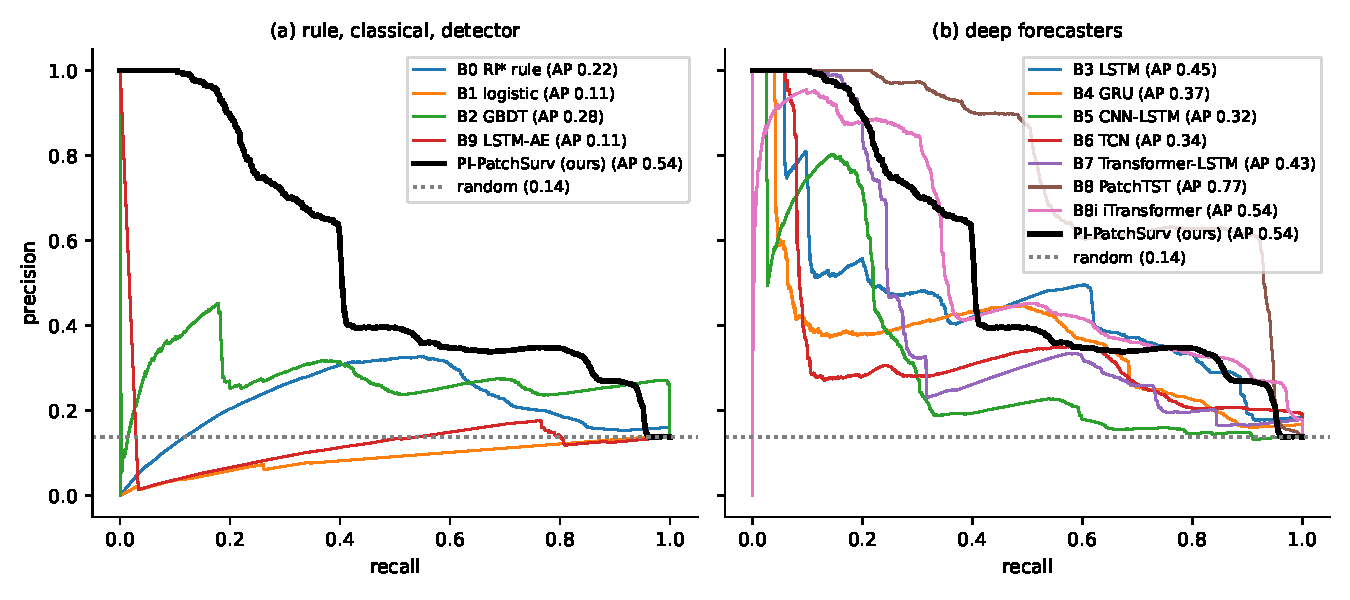
\includegraphics[width=\textwidth]{figures/pr_curves_24h.pdf}
\caption{Precision--recall curves for an event within 24~h, pooled over the six test wells (ensemble of the
available seeds). (a) Physics rule, classical learners and the autoencoder detector; (b) deep forecasters.
The dotted line is the event prevalence.}
\label{fig:pr}
\end{figure*}

\subsection{Deployed alarms}

Ranking does not guarantee a useful alarm, because the threshold has to be fixed before the test well is
seen. Table~\ref{tab:alarms} reports alarms with thresholds chosen on the calibration wells for at most one
false alarm per well-month. With the raw score (\emph{calib}) most models either miss events or raise many
false alarms on the new well, since absolute score levels differ between wells. Subtracting each
instance's own first-hour score (\emph{calib-self}) corrects much of this shift for the recurrent models:
the GRU ensemble improves from 8 to 15 events caught, and the Transformer--LSTM keeps 13--15 events while
its false-alarm rate falls from 0.24 to 0.044 per well-day. For PI-PatchSurv the correction hurts (15 events at
0.26 false alarms per well-day with the raw score, 9 at 0.19 with calib-self). Over seeds, the GRU catches
$14.7\pm1.5$ events at $0.054\pm0.006$ false alarms per well-day and the Transformer--LSTM $13.7\pm0.6$ at
$0.040\pm0.012$; the best single run (tuned GRU) catches 17 of 24 events at 0.052 per well-day with an event
precision of 0.57 and a median lead of 2.9~h. These rates correspond to about 1.2--1.6 false alarms per
well-month, close to but above the target of one. PI-PatchSurv catches $5.8\pm2.9$ events: its score drifts
within the long well-24 instances, which the self-referenced threshold converts into false alarms
(Appendix~\ref{app:extra}). No model false-alarms on the class-6 look-alike (quick restriction of the
choke); hydrate events (classes 8 and 9) are the main confounder, because a downstream plug also raises the
upstream pressure slowly (Table~\ref{tab:faclass}).

\begin{table*}[t]
\caption{Deployed alarms with thresholds fixed on the calibration wells (ensemble of the available seeds; 24 events, about 248 negative well-days). FA: false alarms per negative well-day}\label{tab:alarms}
\footnotesize
\resizebox{\textwidth}{!}{\begin{tabular}{lcccccc}
\toprule
 & \multicolumn{2}{c}{Raw score (calib)} & \multicolumn{4}{c}{Self-referenced score (calib-self)} \\
\cmidrule{2-3}\cmidrule{4-7}
Model & Hits/24 & FA & Hits/24 & FA & Event precision & Lead, h: median (IQR) \\
\midrule
B2 GBDT & 1 & 0.335 & 4 & 0.262 & 0.06 & 31.5 (29.2) \\
B3 LSTM & 17 & 0.254 & 9 & 0.044 & 0.45 & 3.5 (3.6) \\
B4 GRU & 8 & 0.048 & 15 & 0.057 & 0.52 & 3.3 (2.3) \\
B4 GRU (tuned) & 17 & 0.258 & 17 & 0.052 & 0.57 & 2.9 (5.8) \\
B6 TCN & 2 & 0.242 & 1 & 0.073 & 0.05 & 1.3 (0.0) \\
B7 Transformer-LSTM & 13 & 0.238 & 15 & 0.044 & 0.58 & 1.8 (3.5) \\
B7 Transformer-LSTM (tuned) & 10 & 0.077 & 16 & 0.044 & 0.59 & 4.1 (4.4) \\
B8 PatchTST & 19 & 0.214 & 2 & 0.048 & 0.14 & 9.8 (7.7) \\
B8i iTransformer (tuned) & 15 & 0.061 & 14 & 0.105 & 0.35 & 4.7 (4.6) \\
PI-PatchSurv & 15 & 0.262 & 9 & 0.190 & 0.16 & 4.2 (37.1) \\
PI-PatchSurv (tuned) & 14 & 0.198 & 6 & 0.109 & 0.18 & 35.6 (51.3) \\
\bottomrule
\end{tabular}}
\end{table*}


\subsection{Calibration, uncertainty and horizon}

PI-PatchSurv provides the most reliable uncertainty. Its 90\,\% conformal intervals cover 87\,\% of the
test event windows and its median time-to-event error is $\Delta T=6.8$~h, whereas the recurrent models
under-cover (LSTM 0.54, GRU 0.43, Transformer--LSTM 0.33) with $\Delta T$ of 9--24~h; only the
iTransformer reaches similar coverage (0.88) with a larger error (10.0~h). The reliability diagram
(Appendix, Figure~\ref{fig:reliab}) shows that all models over-estimate risk above 0.6, which is expected
when the calibration well holds only one to three events. Figure~\ref{fig:horizon} shows that AUPRC rises
with the horizon for every model, from 0.02--0.33 at 1~h to 0.78--0.93 at 72~h: most windows lie within
a few days of their event, so long horizons are easier, and the short pre-onset records of 3W (median
6.5~h of normal data) cap the useful lead at a few hours.

\begin{figure}[t]
\centering
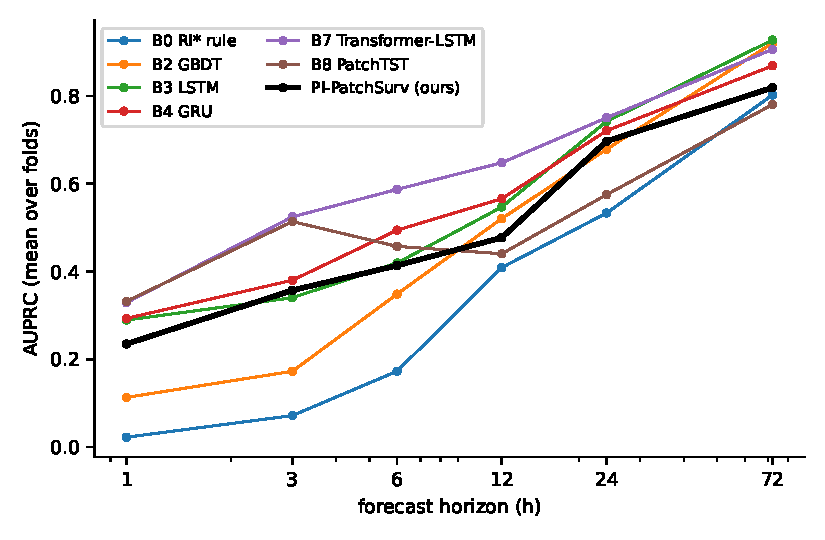
\includegraphics[width=\columnwidth]{figures/horizon_auprc.pdf}
\caption{Horizon sensitivity (E5): AUPRC (mean over folds) against the forecast horizon.}
\label{fig:horizon}
\end{figure}

\subsection{Robustness and generalisation}

Corruptions applied to the test inputs (Appendix~\ref{app:extra}, Table~\ref{tab:robust}) show a clear contrast. PI-PatchSurv is insensitive to sensor loss:
with three of nine sensors replaced by their median and flagged as missing its AUPRC is unchanged
(0.70), whereas the LSTM falls from 0.81 to 0.56 ($-30\,\%$). This follows from the channel-independent,
mask-aware design and is relevant because sensor failure is common in the field. Gaussian noise of up to
5\,\% and an undetected frozen sensor change neither model much. The LSTM is more robust to a change of the
sampling rate (30~s to 5~min, models not retrained) than PI-PatchSurv, whose patch length is tied to the
1-minute grid. In the v1$\to$v2 generalisation test (Appendix~\ref{app:extra}, Table~\ref{tab:v1v2}), where only four events are
available for training, the patch encoder without physics (PatchTST) transfers best (AUPRC 0.61, AUROC
0.92) and PI-PatchSurv reaches 0.28 (AUROC 0.84); the GRU catches 9 of 20 events at 0.05 false alarms per
well-day.


\subsection{Statistical significance}

A Friedman test over the five folds with events is borderline for both the fixed models
($\chi^2=18.2$, $p=0.08$) and the tuned models ($p=0.06$); the Nemenyi critical difference for twelve
models and five folds is 7.45 ranks, and no pair of models differs. Paired instance-level bootstraps with
Holm correction confirm only that PI-PatchSurv outperforms the physics rule, logistic regression and the
autoencoder detector (all $p<0.001$); no difference among the deep forecasters survives correction. With 24
events, 17 of them in one well, the deep models cannot be ranked with confidence, and we do not claim a
winner among them.

\subsection{Qualitative examples}

Figure~\ref{fig:examples} shows two test instances. On the fast-scaling well 24 both PI-PatchSurv and the
GRU follow $\RI$, drop when the restriction temporarily falls after half a day, and rise again before $t_E$.
On the slow-scaling well 22, $\RI$ oscillates for six days; the risk of PI-PatchSurv climbs steadily from
about 0.2 to 0.75, tracking the slow growth, while the GRU switches abruptly from low to high risk about
three days before the event.

\begin{figure*}[t]
\centering
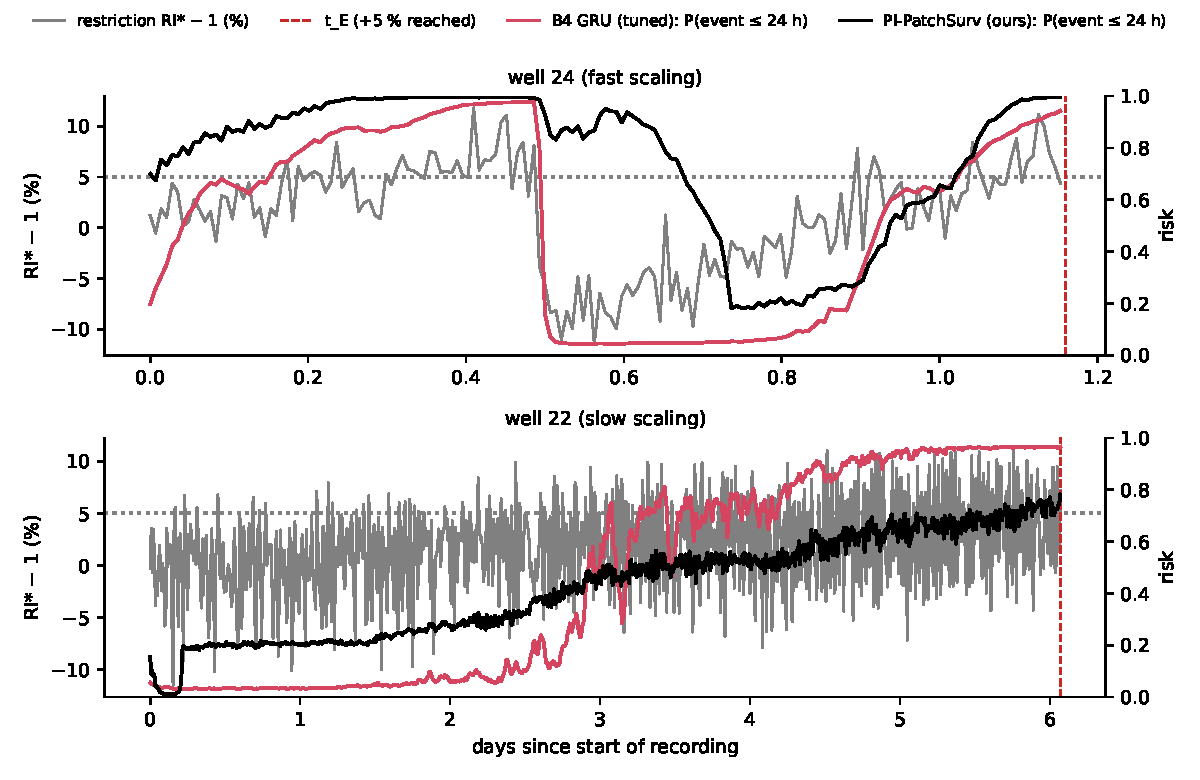
\includegraphics[width=\textwidth]{figures/example_forecasts.pdf}
\caption{Qualitative examples on two unseen test wells: the restriction $\RI-1$ (grey, left axis), the
critical level $+5\,\%$ (dotted) and the forecast risk of an event within 24~h (right axis) of the tuned GRU
and of PI-PatchSurv; the dashed red line marks $t_E$.}
\label{fig:examples}
\end{figure*}

\section{Comparison with base studies and the state of the art}\label{sec:comparison}

The base studies of this work are the 3W dataset papers \citep{vargas2019,vargas2026}, which define the data
and the event classes; the deep-learning detection system of \citet{aranha2024}, whose LSTM autoencoder is
the reference anomaly detector on oil-well sensors; the hybrid Transformer--LSTM of \citet{lai2026}, the
closest forecasting study of a well event with a lead time; PatchTST \citep{nie2023}, on which the sequence
branch of PI-PatchSurv is built; and the open-world detection line of \citet{lopes2025,lopes2026}, which
reports results for choke scaling on 3W. Table~\ref{tab:basepapers} summarises these studies.

\begin{table}[t]
\caption{Base studies: problem, method, data, reported results and main limitations}
\label{tab:basepapers}
\scriptsize\setlength{\tabcolsep}{3pt}
\begin{tabular*}{\textwidth}{@{\extracolsep\fill}p{1.8cm}p{1.7cm}p{2.0cm}p{1.6cm}p{2.2cm}p{2.1cm}}
\toprule
Study & Problem & Method & Data & Reported result & Main limitation \\
\midrule
\citet{vargas2019,vargas2026} & Undesirable-event detection & Dataset and benchmarks & 3W v1 and v2 & Benchmark definitions & No forecasting task \\
\citet{aranha2024} & Anomaly detection & LSTM autoencoder with decision diagram & Field wells, simulated and real & True-positive rate $>$90\,\% in early stages$^*$ & Detection only; split not stated \\
\citet{lopes2025,lopes2026} & Open-world detection and explanation & Autoencoder, classifiers, clustering, LLM agent & Completions; 3W & Novelty detection of choke scaling 94.9\,\% [90.5, 97.3]$^*$ & Detection after onset; not split by well \\
\citet{lai2026} & Timing of water breakthrough & Transformer--LSTM & 9 gas wells, daily data & Breakthrough 2--6 days ahead$^*$ & Other event and field \\
\citet{nie2023} & Long-term forecasting & PatchTST & Public benchmarks & State-of-the-art errors$^*$ & No censoring, no physics \\
\citet{cheng2022} & Scale detection and magnitude & CNN-LSTM-MLP & Simulated histories & $>$95\,\% detection accuracy$^*$ & Simulated data, no timing \\
\botrule
\end{tabular*}
\footnotetext{$^*$Reported in the original study (different task, data or split); not reproduced here.}
\end{table}

\subsection{Quantitative comparison}

The published numbers are not directly comparable with those of this study, because the base studies
address detection or a different event and use different data or splits. To obtain a comparison on the same
data, metrics and protocol, the base architectures were re-implemented (B7 Transformer--LSTM, B8 PatchTST and
B9 LSTM-autoencoder detector) and evaluated exactly as PI-PatchSurv (Table~\ref{tab:quant}).

\begin{table}[t]
\caption{Same-protocol comparison with re-implemented base architectures (leave-one-well-out, 24 events;
mean $\pm$ standard deviation over seeds where several exist). The best deployed baseline is added for
reference}
\label{tab:quant}
\footnotesize\setlength{\tabcolsep}{2.5pt}
\begin{tabular*}{\textwidth}{@{\extracolsep\fill}lccccc}
\toprule
Model & AUPRC@24h & AUROC@24h & Hits/24 & PICP & $\Delta T$ (h) \\
\midrule
B9 LSTM-AE, \citeauthor{aranha2024}$^\dagger$ & 0.262 & 0.365 & 0 & 0.81 & 58.7 \\
B8 PatchTST, \citeauthor{nie2023}$^\dagger$ & $0.569\pm0.041$ & $0.807\pm0.032$ & $2.0\pm1.0$ & 0.52 & 8.8 \\
B7 Transf.--LSTM, \citeauthor{lai2026}$^\dagger$ & $0.711\pm0.031$ & $0.903\pm0.058$ & $13.7\pm0.6$ & 0.33 & 19.6 \\
B4 GRU (best deployed baseline) & $0.712\pm0.123$ & $0.905\pm0.061$ & $14.7\pm1.5$ & 0.43 & 24.2 \\
PI-PatchSurv (proposed) & $0.644\pm0.055$ & $0.794\pm0.018$ & $5.8\pm2.9$ & \textbf{0.87} & \textbf{6.8} \\
\midrule
\citet{lopes2026}, novelty detection$^*$ & \multicolumn{5}{l}{94.9\,\% detection of choke scaling (after onset, not split by well)} \\
\citet{aranha2024}, anomaly detection$^*$ & \multicolumn{5}{l}{True-positive rate $>$90\,\% in early stages (field data)} \\
\botrule
\end{tabular*}
\footnotetext{PICP: coverage of the 90\,\% interval. $^\dagger$Re-implemented and evaluated under the protocol of this study. $^*$Taken from the original study; different task and split, shown for context only.}
\end{table}

Against the re-implemented autoencoder detector, PI-PatchSurv improves AUPRC@24h by 0.382 (146\,\% relative)
and AUROC by 0.429; the gain comes from changing the objective from reconstruction to time-to-event.
Against PatchTST it improves AUPRC by 0.075 (13\,\%), catches 3.8 more events and raises interval coverage
from 0.52 to 0.87; the ablation study attributes this gain to the physics branch and the survival head.
Against the Transformer--LSTM it is lower in AUPRC (by 0.067, or 9\,\%), in AUROC (by 0.109) and in events
caught (by 7.9), but it reduces the time-to-event error from 19.6 to 6.8~h (65\,\%) and raises coverage from
0.33 to 0.87. None of the differences among the deep forecasters is statistically significant
(Section~\ref{sec:significance}).

\subsection{Methodological comparison}

The base detectors model normal operation and flag deviations from it. They answer whether an event is
present, not when it becomes critical, and B9 confirms that a reconstruction score carries almost no
information about the time to the critical level (AUROC 0.37). PatchTST and the Transformer--LSTM forecast
continuous series, but neither handles censoring nor uses process physics. PI-PatchSurv differs from them
in its objective, a censoring-aware survival likelihood with a monotone risk curve; in its inputs, a
self-referenced restriction proxy and physics trends fused through a gate; in its training, which adds
synthetic instances, a monotonicity loss and a deep ensemble; and in its deployment, which uses
self-referenced thresholds and conformal intervals calibrated on separate wells.

\subsection{Fairness of the comparison}

Five factors limit the comparison. First, the published numbers come from detection tasks, from other events
such as water breakthrough or from other data such as completion faults and simulated scale histories, and
most use random or sample-level splits; a held-out-well protocol on 3W lowers macro-F1 from 0.99 to 0.30
\citep{issue231}. Second, the base architectures were re-implemented with the inputs, budget and early
stopping of this study rather than their original hyper-parameters, which Optuna tuning under an equal
budget partly offsets (Appendix~\ref{app:extra}). Third, several publisher pages were not accessible, so only
results stated in accessible abstracts or preprints are quoted. Fourth, seed 0 and seeds 1--2 were trained
on different hardware (Apple M4 and NVIDIA T4), which adds a small amount of variance. Fifth, PI-PatchSurv
does not outperform the best recurrent baselines in ranking or in deployed recall; its advantages are the
quality of its uncertainty, the accuracy of its time-to-event estimate and its robustness to missing sensors.

\section{Ablation study}\label{sec:ablation}

Table~\ref{tab:ablation} and Fig.~\ref{fig:ablation} report the effect of removing or modifying one
component of PI-PatchSurv at a time. The ablations of the physics branch, the survival head and the
synthetic data were run with three seeds, the chemistry prior and the tuned model with five, and the
remaining variants with one seed.

\begin{table*}[t]
\caption{Ablation of PI-PatchSurv. $\Delta$: reference minus variant on pooled AUPRC@24h (paired instance bootstrap, 95\,\% CI, Holm-corrected $p$).}\label{tab:ablation}
\scriptsize\setlength{\tabcolsep}{3pt}
\resizebox{\textwidth}{!}{\begin{tabular}{lccccccc}
\toprule
Variant & Seeds & AUPRC@24h & AUROC@24h & C-index & ECE & Hits/24 & $\Delta$ pooled AUPRC [CI], $p$ \\
\midrule
Full model (reference) & 5 & 0.644$\pm$0.055 & 0.794$\pm$0.018 & 0.802 & 0.234 & 5.8$\pm$2.9 & -- \\
$-$ physics branch & 3 & 0.581$\pm$0.036 & 0.718$\pm$0.002 & 0.730 & 0.295 & 7.0$\pm$3.0 & +0.068 [-0.05, +0.22], 1.00 \\
$-$ $\mathcal{L}_{\mathrm{mono}}$ & 1 & 0.664 & 0.771 & 0.750 & 0.243 & 4 & +0.005 [-0.04, +0.05], 1.00 \\
$-$ survival head (per-horizon BCE) & 3 & 0.682$\pm$0.030 & 0.842$\pm$0.045 & 0.778 & 0.155 & 3.0$\pm$1.7 & -0.231 [-0.39, -0.07], 0.27 \\
$-$ patching (patch length 1) & \multicolumn{7}{c}{not available} \\
patch 8, no overlap & 1 & 0.681 & 0.780 & 0.742 & 0.171 & 7 & -0.038 [-0.11, +0.04], 1.00 \\
$-$ synthetic training data & 3 & 0.654$\pm$0.032 & 0.911$\pm$0.001 & 0.754 & 0.247 & 9.3$\pm$2.5 & +0.217 [+0.08, +0.36], 0.07 \\
$+$ PHREEQC SI prior & 5 & 0.657$\pm$0.034 & 0.792$\pm$0.020 & 0.792 & 0.191 & 5.0$\pm$2.7 & -0.060 [-0.12, +0.01], 1.00 \\
Optuna-tuned & 5 & 0.596$\pm$0.093 & 0.746$\pm$0.076 & 0.765 & 0.285 & 5.6$\pm$2.9 & -0.009 [-0.13, +0.13], 1.00 \\
\bottomrule
\end{tabular}}
\end{table*}


\begin{figure}[t]
\centering
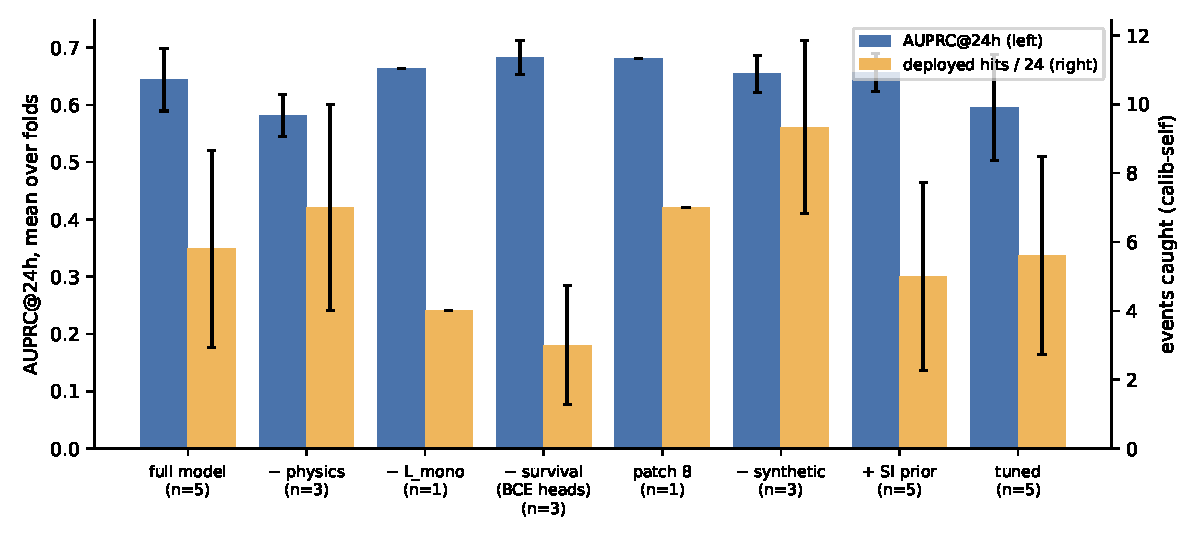
\includegraphics[width=0.7\textwidth]{figures/ablation_bars.pdf}
\caption{Ablation results: AUPRC@24h (left axis) and events caught with the deployed threshold (right axis).
Bars show the mean and whiskers one standard deviation over $n$ seeds}
\label{fig:ablation}
\end{figure}

The physics branch is the component with the clearest effect. Removing it lowers AUROC from
$0.794\pm0.018$ to $0.718\pm0.002$, the C-index from 0.80 to 0.73 and AUPRC from 0.644 to $0.581\pm0.036$,
and it worsens calibration (ECE from 0.23 to 0.30). The effect is consistent across seeds, which indicates
that the engineered restriction trends carry information that the patch encoder does not recover from 24
events alone.

Replacing the survival head by independent per-horizon classifiers gives a slightly higher AUPRC
($0.682\pm0.030$) and a higher pooled AUPRC (0.80 against 0.54), but fewer events caught under the deployed
threshold ($3.0\pm1.7$ against $5.8\pm2.9$), lower interval coverage (0.59 against 0.87) and risk curves
that are no longer guaranteed to increase with the horizon. Choosing between the two on the test wells would
amount to test-set selection, so the survival head is kept by design and the trade-off is reported.

Training on real instances only raises AUROC ($0.911\pm0.001$) and the number of deployed events
($9.3\pm2.5$), but pooled AUPRC falls from 0.54 to 0.34 and interval coverage from 0.87 to 0.45. The
simulated and hand-drawn instances therefore mainly make scores comparable across wells and calibrate the
time-to-event estimate, rather than improving the ranking within a well.

Removing patching (patch length 1, so that every minute becomes a token) lowers AUPRC from 0.726 to 0.628
and AUROC from 0.790 to 0.740 relative to the same seed of the full model, while raising the number of
tokens per channel from 44 to 360 and the training cost accordingly; a patch length of 8 without overlap
changes little. Removing the monotonicity loss is neutral in ranking but reduces the number of deployed
events. The PHREEQC saturation-index prior gives small, non-significant gains (AUPRC $0.657\pm0.034$, pooled
AUPRC 0.60, PICP 0.89); because the brines are a regional average rather than the wells' own water, this is
a lower bound on what chemistry can add. Finally, Optuna tuning on the calibration-well loss did not help
PI-PatchSurv ($0.596\pm0.093$), since the tuning objective is noisy when it rests on one small calibration
well.

\section{Discussion}\label{sec:discussion}

\textbf{Why the approach works, and where it does not.} The decisive step is the formulation:
self-referencing the restriction to each instance's own baseline turns wells of very different pressure
into one learnable problem, and the survival objective uses the many censored windows instead of
mislabelling them. Every learned forecaster built on this formulation outperforms the physics rule and the
anomaly detector. Within the deep models, the recurrent architectures rank and alarm best: the informative
signal is a slow trend in two or three channels, which a recurrent state integrates directly, whereas a
patch Transformer splits it into 16-minute tokens and must re-assemble it through attention from only 24
positive events. The physics branch, the mask-aware channel-independent encoder and the ensemble give
PI-PatchSurv properties that matter in operation, namely calibrated intervals, an accurate time-to-event
and robustness to failed sensors, but not a better ranking.

\textbf{Practical implications.} With a threshold fixed on other wells, the best forecasters warn of
roughly two thirds of the events a median of 2--4~h before the restriction reaches $+5\,\%$, at 1.2--1.6
false alarms per well-month, and they raise no alarm on normal operation or on the quick-restriction
look-alike. Hours of warning are enough to schedule a choke cleaning within a shift but not to plan an
inhibitor campaign; longer warnings require longer real histories than 3W provides. Self-referencing the
score to each well's own recent level is a simple, model-agnostic step that roughly doubles deployed recall
for several models and should be part of any deployment.

\textbf{Strengths.} The study evaluates on wells excluded from training with all thresholds and
hyper-parameters chosen on separate calibration wells; it compares twelve models with fixed and tuned
hyper-parameters and several seeds; it reports calibration, intervals, event-level and confounder-level
false alarms, robustness and a dataset-version generalisation test; and every number is regenerated from
saved predictions by published code.

\textbf{Failure cases.} (i) On well 24, PI-PatchSurv's score drifts within long instances and produces
false alarms under the self-referenced threshold. (ii) Hydrate plugs downstream of the choke (classes 8 and
9) raise the upstream pressure slowly and are confused with scale; separating them needs the missing
downstream sensors or temperature dynamics. (iii) Wells 6 and 21 contribute few events and are often
missed. (iv) The autoencoder detector does not forecast at all.

\textbf{Threats to validity.} \emph{Internal:} only 24 real events are available and 17 come from one well,
so fold-level variance is large and the deep models cannot be separated statistically; ablations other than
three components use a single seed. \emph{Construct:} $\RI$ is a proxy based on one pressure and does not
control for changes of the choke opening, which is missing in most instances; the $+5\,\%$ level is a
modelling choice. \emph{External:} 3W covers offshore wells of one operator with short recordings;
results may differ for onshore gas wells or other scale chemistries. \emph{Conclusion validity:}
early stopping and tuning rely on a single small calibration well per fold, which makes both noisy.

\textbf{Were the research gap and objectives met?} The first gap, the absence of timed forecasting of
scaling, is addressed: calibrated multi-horizon forecasts on unseen wells are shown to be feasible, but the
lead time is hours, not the days targeted in the proposal, because of the data. The second gap, the lack of
fusion of chemistry and sensors, is addressed only partly: physical indicators are fused with learned
features and help, while the chemistry prior from public brines helps little. The third gap, the absence of
unseen-well evaluation, is fully addressed. The fourth gap, rare events and missing uncertainty, is
addressed by censor-aware training, synthetic data and conformal intervals with near-nominal coverage. The
objective of a proposed model that outperforms all baselines was not achieved; the evidence instead
supports the formulation and the evaluation protocol, with simple recurrent forecasters as the strongest
rankers.

\section{Conclusion and future work}\label{sec:conclusion}

This paper formulated the forecasting of mineral-scale restriction in production chokes as a
discrete-time survival problem on production-sensor data, introduced a self-referenced restriction proxy,
proposed the physics-informed survival model PI-PatchSurv, and benchmarked twelve models on unseen wells of
the 3W dataset. Learned forecasters clearly outperform a physics threshold rule and an anomaly detector;
recurrent models rank and alarm best, catching about two thirds of the events hours ahead at 1.2--1.6
false alarms per well-month, while PI-PatchSurv provides the best-calibrated uncertainty, the most accurate
time-to-event and robustness to sensor loss. Future work should (i) evaluate the formulation on field data
with long histories, cleaning logs and water analyses to reach multi-day warnings; (ii) add per-well domain
adaptation so that thresholds transfer without self-referencing; (iii) separate hydrate from scale events
with temperature dynamics or downstream sensors; (iv) combine survival and per-horizon objectives in one
head selected on calibration wells; and (v) contribute a time-to-restriction benchmark to the 3W repository.


\backmatter
\section*{Declarations}\label{sec:declarations}

\bmhead{Data availability}
The 3W dataset v2.0.0 is publicly available under the CC BY 4.0 licence from the Petrobras repository
\cite{petrobras3w} (commit \texttt{826fec4} was used). The produced-water analyses used for the chemistry
prior are available from the U.S. Geological Survey~\cite{blondes2023}.

\bmhead{Code availability}
The complete code (preprocessing, models, training, evaluation, figures and tables), the run logs, the
tuned hyper-parameters and all result tables are available at
\url{https://github.com/i257608-cmd/scale-forecasting}. The saved model predictions (143~MB) are available
from the corresponding author on request; from them, two commands (\texttt{python experiments/analyze.py} and
\texttt{python scripts/paper\_tables.py}) regenerate every number, table and figure of this paper, and the
full pipeline in the repository regenerates the predictions themselves.

\bmhead{Funding}
This research received no external funding.

\bmhead{Conflict of interest}
The authors declare no competing interests.

\bmhead{Author contributions}
M.H.: conceptualisation, methodology, software, experiments, writing. M.S.: methodology, validation,
writing -- review and editing.

\bmhead{Use of AI-assisted tools}
An AI assistant (Anthropic Claude) was used to help write and debug code, run and monitor experiments,
search and check literature metadata, and draft and edit the text of this paper. All experiments were run
on the authors' machines and accounts, every reported number is produced by the published code from the
saved predictions, and the authors reviewed and take full responsibility for the content.

\bmhead{Acknowledgements}
The authors thank Petrobras and the 3W community for releasing the dataset, and the course instructor for
feedback on the research proposal.


\bibliography{references}

\begin{appendices}
\section{Additional results}\label{app:extra}

Table~\ref{tab:tuned} repeats Table~\ref{tab:main} with Optuna-tuned hyper-parameters. Tuning improved the
deployed alarms of the GRU and the Transformer--LSTM and reduced those of the LSTM, CNN-LSTM, TCN and
PatchTST; tuning on a single small calibration well mainly adds variance. Table~\ref{tab:faclass} lists false
alarms per confounder class, Table~\ref{tab:robust} the robustness tests and Table~\ref{tab:v1v2} the
generalisation from 3W version 1.1.1 to version 2.0.0. Figures~\ref{fig:reliab} and~\ref{fig:lead} show the
calibration of the forecasts and the lead times of caught events.

\begin{table*}[t]
\caption{As Table~\ref{tab:main}, with Optuna-tuned hyper-parameters (equal budget, tuned on calibration wells).}\label{tab:tuned}
\scriptsize\setlength{\tabcolsep}{3pt}
\resizebox{\textwidth}{!}{\begin{tabular}{lcccccccccc}
\toprule
Model & Seeds & AUPRC@24h & AUROC@24h & C-index & IBS & ECE & BSS & Rec.@1/mo & Hits/24 & PICP \\
\midrule
{B1 Logistic regression} & 1 & 0.281 & 0.406 & 0.434 & 0.366 & 0.529 & 0.26 & 0.04 & 0 & 0.94 \\
{B2 GBDT} & 1 & 0.662 & 0.893 & 0.786 & 0.081 & 0.217 & 0.68 & 0.71 & 6 & 0.72 \\
{B3 LSTM} & 1 & 0.776 & 0.917 & 0.855 & 0.103 & 0.197 & 0.72 & 0.12 & 2 & 0.45 \\
{B4 GRU} & 1 & 0.668 & 0.902 & 0.890 & 0.100 & 0.204 & 0.76 & 0.71 & 17 & 0.41 \\
{B5 CNN-LSTM} & 1 & 0.689 & 0.897 & 0.818 & 0.125 & 0.215 & 0.70 & 0.08 & 5 & 0.53 \\
{B6 TCN} & 1 & 0.762 & 0.940 & 0.879 & 0.116 & 0.190 & 0.77 & 0.12 & 7 & 0.46 \\
{B7 Transformer-LSTM$^\dagger$} & 1 & 0.752 & 0.930 & 0.869 & 0.067 & 0.126 & 0.85 & 0.79 & 16 & 0.70 \\
{B8 PatchTST$^\dagger$} & 1 & 0.616 & 0.827 & 0.849 & 0.149 & 0.198 & 0.75 & 0.67 & 11 & 0.53 \\
{B8i iTransformer} & 1 & 0.700 & 0.935 & 0.820 & 0.091 & 0.157 & 0.78 & 0.46 & 14 & 0.60 \\
{B9 LSTM-AE detector$^\dagger$} & 1 & 0.211 & 0.312 & 0.431 & 0.765 & 0.848 & -0.93 & 0.00 & 0 & 0.85 \\
{PI-PatchSurv (ours)} & 5 & 0.596$\pm$0.093 & 0.746$\pm$0.076 & 0.765 & 0.105 & 0.285 & 0.64 & 0.25 & 5.6$\pm$2.9 & 0.86 \\
\bottomrule
\end{tabular}}
\footnotetext{AUPRC/AUROC and hits: mean$\pm$SD over single-seed runs where several seeds exist; other columns: ensemble of the available seeds. BSS: Brier skill score at 24~h relative to B0. Rec.@1/mo: threshold-free recall at one false alarm per well-month. Hits: events caught out of 24 with the deployed calib-self threshold. PICP: coverage of the 90\,\% conformal interval. $^\dagger$Re-implementation of a base-paper architecture.}
\end{table*}

\begin{table}[t]
\caption{False-alarm episodes per confounder class (calib-self; all real non-scaling instances tested once); $^\ddagger$tuned}\label{tab:faclass}
\scriptsize
\begin{tabular*}{\columnwidth}{@{\extracolsep\fill}lccccc}
\toprule
Class & Inst. & B2 & B4$^\ddagger$ & B7$^\ddagger$ & Ours \\
\midrule
0 normal & 594 & 50 & 0 & 3 & 3 \\
6 quick restr. & 6 & 0 & 0 & 0 & 0 \\
8 hydrate (prod.) & 14 & 3 & 2 & 1 & 21 \\
9 hydrate (serv.) & 57 & 8 & 6 & 3 & 12 \\
3 slugging & 32 & 0 & 0 & 0 & 9 \\
1, 2, 4, 5 & 380 & 4 & 5 & 4 & 2 \\
\bottomrule
\end{tabular*}
\end{table}

\begin{table}[t]
\caption{Robustness (E3): AUPRC@24h under corruptions of the test inputs.}\label{tab:robust}
\scriptsize
\begin{tabular*}{\columnwidth}{@{\extracolsep\fill}lcc}
\toprule
Condition & PI-PatchSurv & B3 LSTM \\
\midrule
clean & 0.697 & 0.811 \\
Gaussian noise 1\,\% & 0.696 & 0.808 \\
Gaussian noise 3\,\% & 0.683 & 0.793 \\
Gaussian noise 5\,\% & 0.674 & 0.773 \\
1 sensor dropped & 0.714 & 0.682 \\
2 sensors dropped & 0.725 & 0.613 \\
3 sensors dropped & 0.700 & 0.564 \\
1 sensor frozen 60 min & 0.699 & 0.796 \\
resampled to 30 s & 0.653 & 0.824 \\
resampled to 60 s & 0.635 & 0.814 \\
resampled to 120 s & 0.611 & 0.787 \\
resampled to 300 s & 0.581 & 0.765 \\
\bottomrule
\end{tabular*}
\end{table}

\begin{table}[t]
\caption{Generalisation: trained on wells of 3W v1.1.1, tested on wells added in v2.0.0 (20 events)}\label{tab:v1v2}
\scriptsize
\begin{tabular}{lccc}
\toprule
Model & AUPRC@24h & AUROC@24h & Hits/20 / FA \\
\midrule
B0 & 0.194 & 0.704 & 0 / 0.261 \\
B2 & 0.227 & 0.693 & 2 / 0.174 \\
B3 & 0.475 & 0.834 & 3 / 0.112 \\
B4 & 0.358 & 0.690 & 9 / 0.050 \\
B5 & 0.339 & 0.776 & 0 / 0.062 \\
B6 & 0.185 & 0.702 & 0 / 0.075 \\
B7 & 0.166 & 0.683 & 0 / 0.000 \\
B8 & 0.605 & 0.922 & 1 / 0.485 \\
B8i & 0.264 & 0.822 & 0 / 0.137 \\
B9 & 0.097 & 0.447 & 0 / 0.050 \\
PI-PatchSurv & 0.278 & 0.841 & 4 / 0.373 \\
\bottomrule
\end{tabular}
\end{table}


\begin{figure}[t]
\centering
\begin{minipage}{0.46\textwidth}
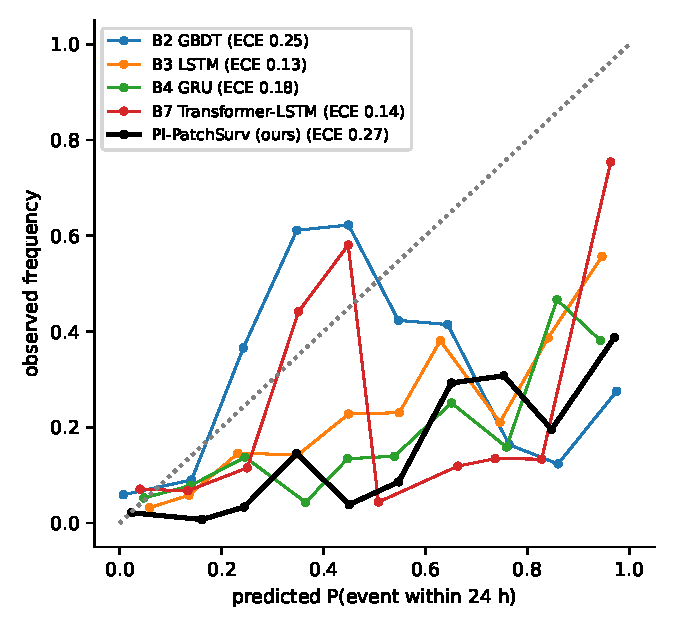
\includegraphics[width=\linewidth]{figures/reliability_24h.pdf}
\caption{Reliability diagram for an event within 24~h (pooled test wells) with the expected calibration error}
\label{fig:reliab}
\end{minipage}\hfill
\begin{minipage}{0.52\textwidth}
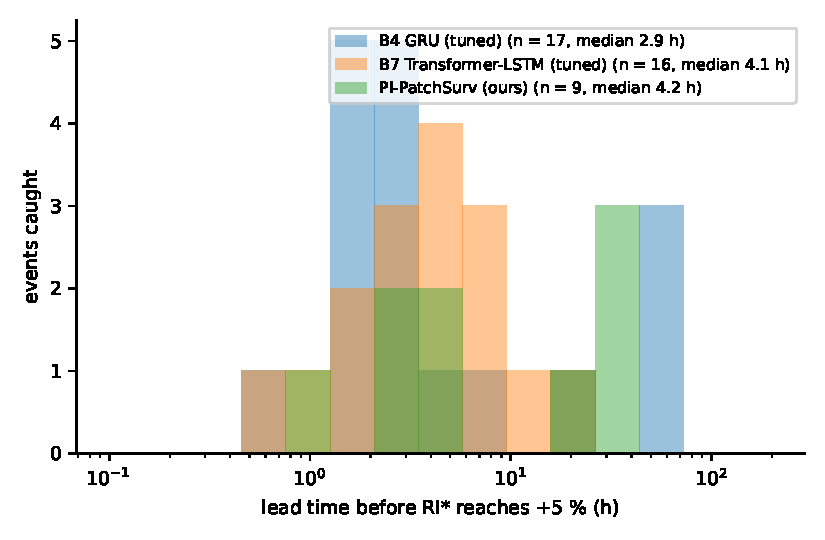
\includegraphics[width=\linewidth]{figures/lead_time_hist.pdf}
\caption{Lead time of caught events under the deployed self-referenced threshold}
\label{fig:lead}
\end{minipage}
\end{figure}

\section{Reproducibility details}\label{app:repro}

Table~\ref{tab:repro} lists the settings needed to reproduce the experiments.

\begin{table}[h]
\caption{Settings used in all experiments}
\label{tab:repro}
\footnotesize
\begin{tabular*}{\textwidth}{@{\extracolsep\fill}p{2.2cm}p{9.8cm}}
\toprule
Item & Setting \\
\midrule
Data & 3W v2.0.0, commit \texttt{826fec4}; onset = first label 107 or 7; event when the 60-min rolling median of $\RI$ reaches 1.05; windows of 360~min every 10~min; horizons 1, 3, 6, 12, 24 and 72~h \\
Splits & Six leave-one-well-out folds (test wells 1, 6, 21, 22, 23, 24); calibration well = next scaling well with an event, never well 24; non-scaling wells rotate into test and calibration groups; v1$\to$v2: train on wells 1, 6 and 21, test on 22--24, calibrate on 6 \\
Hyper-parameters & $d=64$; AdamW, learning rate $10^{-3}$, weight decay $10^{-4}$; batch 256; 12 epochs of 150 steps; dropout 0.1; Transformer with 2 layers, 4 heads, feed-forward width 128; patch 16, stride 8; $\lambda=0.1$; recurrent baselines with 2 layers \\
Tuning & Optuna 5.0, TPE sampler (seed 0), median pruner, 20 trials per fold, 4 epochs per trial; learning rate $[10^{-4},3\cdot10^{-3}]$ (log), weight decay $[10^{-6},10^{-2}]$ (log), batch $\{128,256,512\}$, $\lambda\in[0,0.5]$ (PI-PatchSurv) \\
Seeds & 0--4 for PI-PatchSurv, its \emph{-SI} and tuned variants; 0--2 for deep baselines and the physics, survival-head and synthetic-data ablations; 0 for other variants \\
Environment & Python 3.14.7, PyTorch 2.15.0, NumPy 2.5, pandas 3.1, scikit-learn 1.9.1, SciPy 1.18, Optuna 5.0; Apple M4 (MPS, float32) and Kaggle with two NVIDIA T4 GPUs (CUDA) \\
Commands & \texttt{python experiments/analyze.py}, \texttt{python experiments/analyze.py --split v1v2} and \texttt{python scripts/paper\_tables.py} regenerate all tables and figures; \texttt{scripts/phase2\_queue.sh} runs the full training pipeline \\
\botrule
\end{tabular*}
\end{table}

\end{appendices}

\end{document}
